\documentclass{beamer}

%\usepackage{multimedia}

% For more themes, color themes and font themes, see:
% http://deic.uab.es/~iblanes/beamer_gallery/index_by_theme.html
%
\mode<presentation>
{
  \usetheme{Madrid}       % or try default, Darmstadt, Warsaw, ...
  \usecolortheme{seahorse} % or try albatross, beaver, crane, ...
  \usefonttheme{serif}    % or try default, structurebold, ...
  \setbeamertemplate{navigation symbols}{}
  \setbeamertemplate{caption}[numbered]
	\setbeamertemplate{footline}{}
	\setbeamersize{text margin right=2pt}
} 

\usepackage{tikz}
\usetikzlibrary{decorations.markings,angles}
\usepackage{tikz-3dplot} 

\usepackage{amsmath}


\begin{document}

\begin{frame}{Different time behaviour}

\vspace{-0.8cm}

\begin{figure}[H]
 \centering
 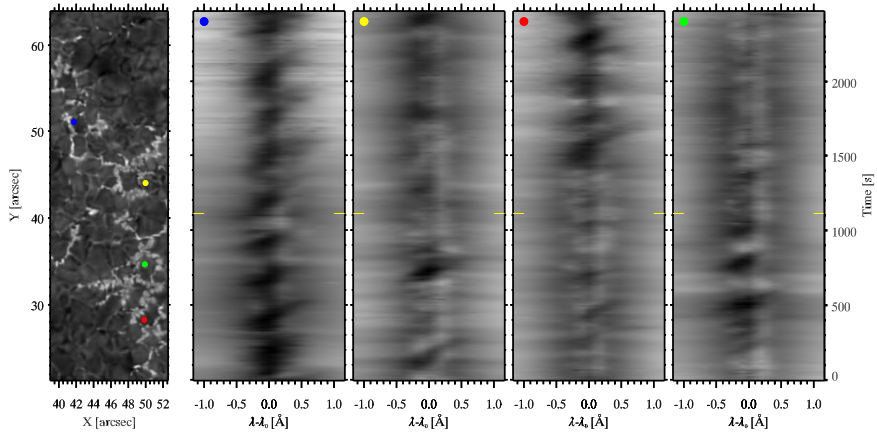
\includegraphics[scale=0.4]{im1.png}
\caption{ The second panel from left corresponds to a traditional absorption profile showing a
shock-induced temporal pattern. The last three panels correspond to the time evolution of three RC profiles. The time of the image in the top left panel is indicated
in the time slices with a yellow marker.}
\end{figure}

\end{frame}

\begin{frame}{Different time behaviour - No RC profile}
\begin{minipage}{0.59\linewidth}
\begin{figure}[H]
 \centering
 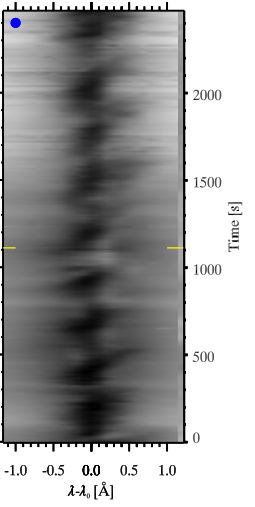
\includegraphics[scale=0.4]{im1-p2t.png}
\end{figure}
\end{minipage}	
\begin{minipage}{0.39\linewidth}
\begin{itemize}
\item succession of MHD shocks (characteristic strong absorption features)
\item 2 brief RC moments between shocks
\end{itemize}
\end{minipage}	

\end{frame}

\begin{frame}{Different time behaviour - RC profile}
\vspace{-0.8cm}
\begin{minipage}[l]{0.69\linewidth}
\begin{figure}[H]
 \centering
 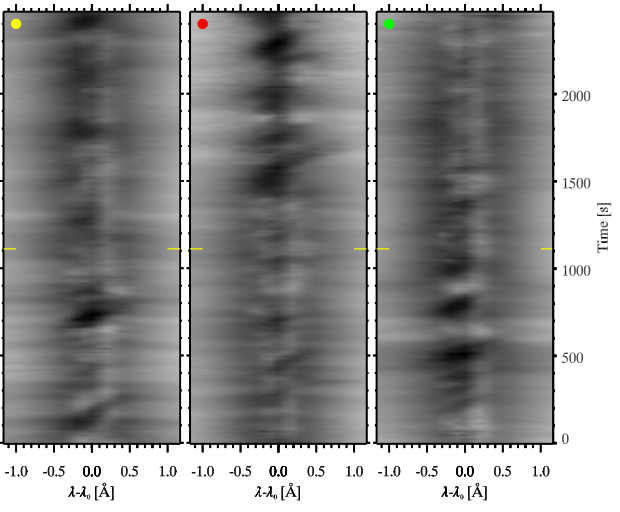
\includegraphics[scale=0.4]{im1-p3-5.png}
\end{figure}
\end{minipage}	
\begin{minipage}[r]{0.29\linewidth}
\begin{itemize}
\item RC emission for most of the series
\item occasional shock induced absorption
\item imprint of red emission lobe at +194 $m\AA$  noticeable throughout time series, but not for the blue lobe
\end{itemize}
\end{minipage}	

\end{frame}


\begin{frame}{Frames from Fig.2 animation movie}

%\movie[height = 0.6\textwidth, width = 0.8\textwidth, poster, showcontrols] {}{video.avi}

\begin{figure}[H]
 \centering
 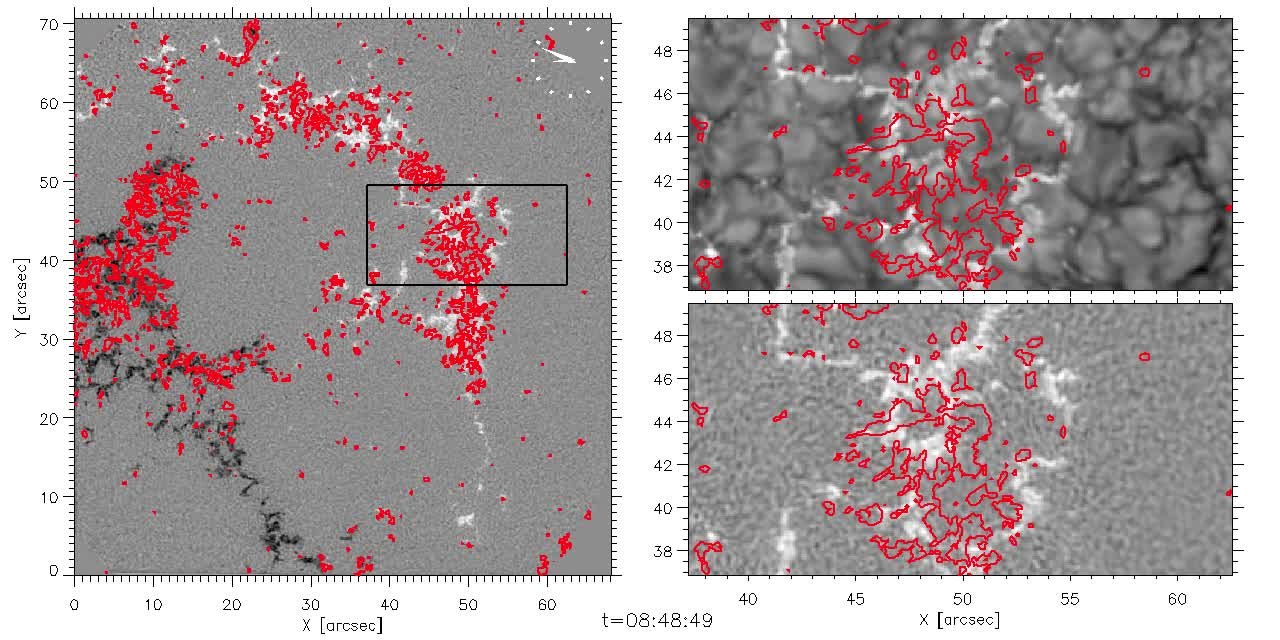
\includegraphics[scale=0.28]{output006.jpg}
\end{figure}

\end{frame}
\begin{frame}{Frames from Fig.2 animation movie}

\begin{figure}[H]
 \centering
 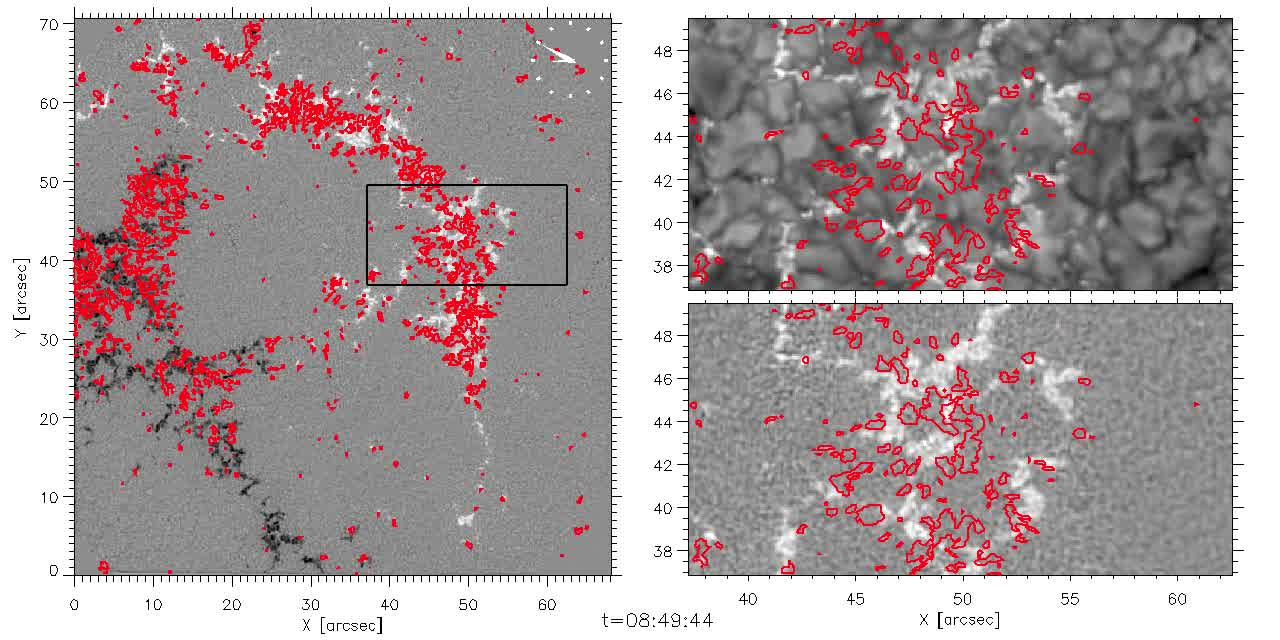
\includegraphics[scale=0.28]{output007.jpg}
\end{figure}

\end{frame}
\begin{frame}{Frames from Fig.2 animation movie}
\begin{figure}[H]
 \centering
 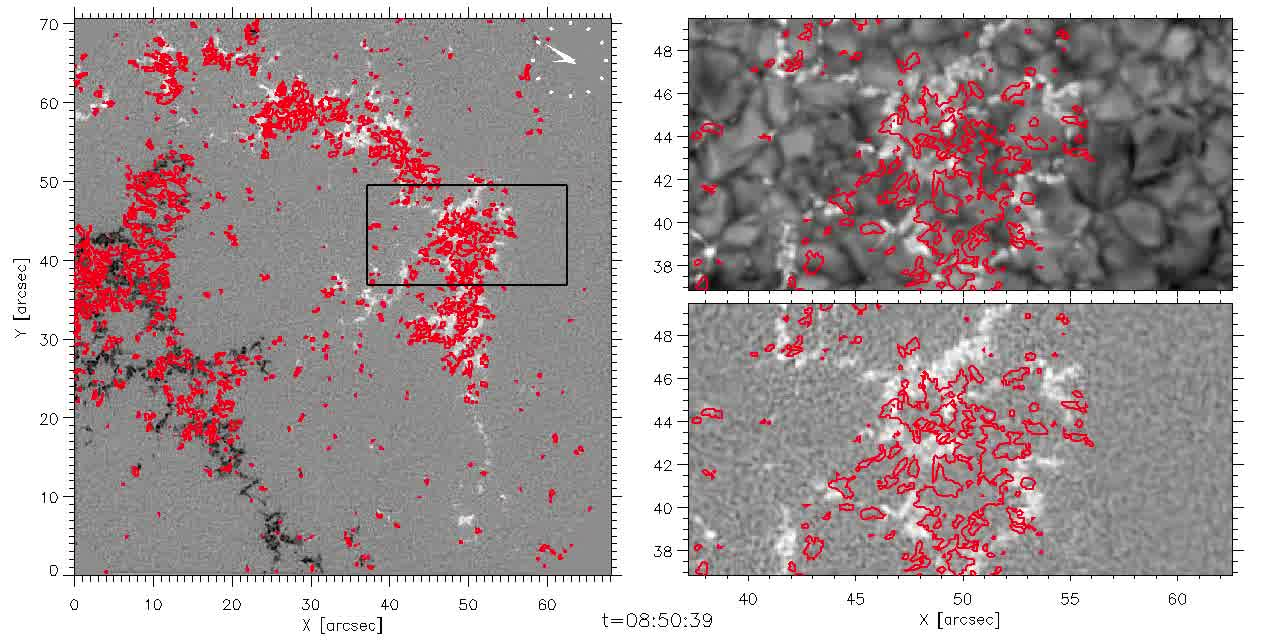
\includegraphics[scale=0.28]{output008.jpg}
\end{figure}

\end{frame}

\begin{frame}{Frames from Fig.2 animation movie}
\begin{figure}[H]
 \centering
 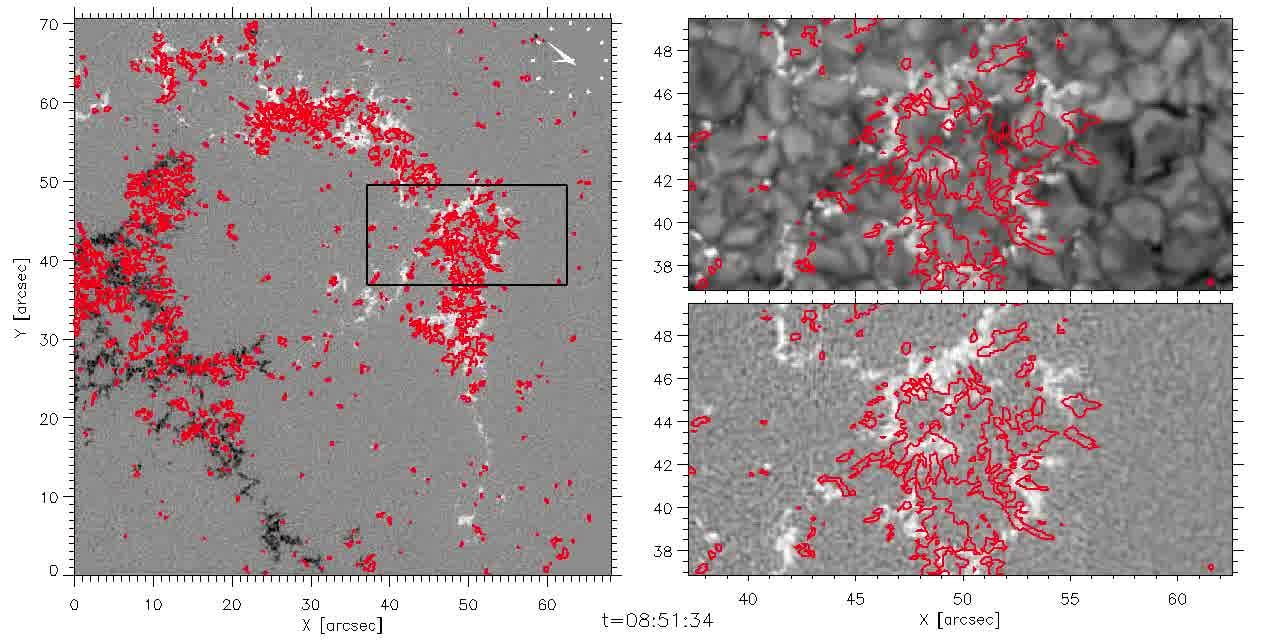
\includegraphics[scale=0.28]{output009.jpg}
\end{figure}

\end{frame}

\begin{frame}{Frames from Fig.2 animation movie}
\begin{itemize}
\item contiguous and/or coherent spatial regions
that contain RC profiles with typical spatial and temporal scales
of the order of 0.5 arcsec and 1-2 minutes. 
\item These regions change shape
and move about within the plage region
\end{itemize}
\end{frame}


\begin{frame}{Autocovariance timescale}


\begin{equation*}
f(\vec{x},t) = 
\begin{cases}
1 \text{ if the point } \vec{x} \text{ has a RC profile:} \\ \hspace{1.5cm} \text{ number of zero-crossings of } 
\frac{d I}{d \lambda}(\vec{x},t) > 1, \\
0 \text{ if the point } \vec{x} \text{ does not have a RC profile:} \\ \hspace{1.5cm} \text{ number of zero-crossings of } 
\frac{d I}{d \lambda}(\vec{x},t) = 1 
\end{cases}
\end{equation*}

\begin{itemize}
\item autocovariance timescale at $\vec{x}$ = $FWHM(f(\vec{x},t),t)$
\item seeing deformations, jitter, and proper motions have {\bf smaller } lifetimes than points with RC profile
\item remove these effects by rebinning the data starting from 1x1 to 16x16 pixels (timescale increases until there is no more difference
from 8x8 to 16x16 pixels both showing a timescale of 80s)
\item timescale 1-2 minutes and spatial scale 8 pixels (0.5 arcsec)
\end{itemize}

\end{frame}


\begin{frame}{Autocovariance timescale}
\vspace{-0.3cm}
\begin{figure}[H]
 \centering
 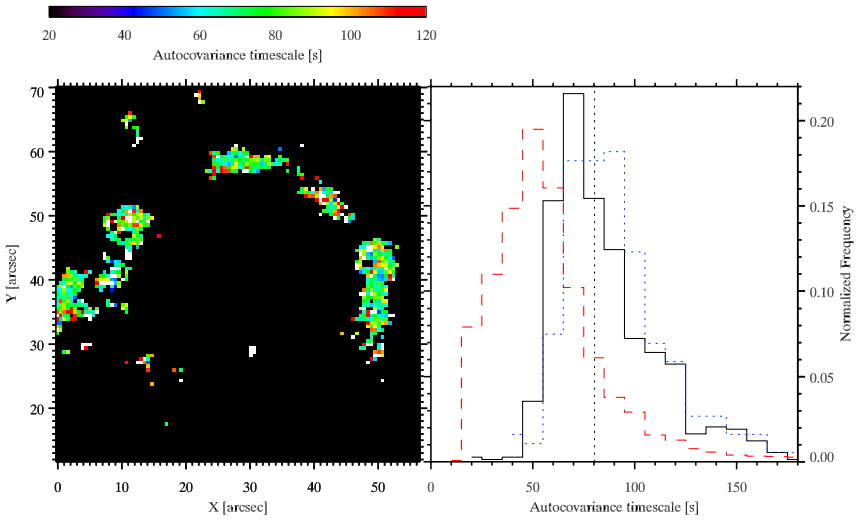
\includegraphics[scale=0.35]{im2.png}
	\caption{\small {\bf Left:} map of the autocovariance timescale (8x8 rebinned) 
	{\bf Right:}  a histogram of autocovariance timescales for locations with RC profiles, using the original data
(dashed-red), 8x8 (solid-black), and 16x16 rebinning (dotted-blue). 
The vertical black-dotted line indicates the median autocovariance timescale:81s.}
\end{figure}

\end{frame}
\end{document}
